\documentclass[submit]{harvardml}

\course{CS181-S22}
\assignment{Assignment \#4}
\duedate{11:59pm EST, March 25, 2022} 

\usepackage[OT1]{fontenc}
\usepackage[colorlinks,citecolor=blue,urlcolor=blue]{hyperref}
\usepackage[pdftex]{graphicx}
\usepackage{graphicx}
\usepackage{caption}
\usepackage{fullpage}
\usepackage{soul}
\usepackage{amsmath}
\usepackage{framed}
\usepackage{amssymb}
\usepackage{color}
\usepackage{todonotes}
\usepackage{listings}
\usepackage{common}

\usepackage[mmddyyyy,hhmmss]{datetime}

\definecolor{verbgray}{gray}{0.9}

\lstnewenvironment{csv}{
  \lstset{backgroundcolor=\color{verbgray},
  frame=single,
  framerule=0pt,
  basicstyle=\ttfamily,
  columns=fullflexible}}{}
 
\begin{document}

\begin{center}
{\Large Homework 4: SVM, Clustering, and Ethics}\\
\end{center}

\subsection*{Introduction}

This homework assignment will have you work with SVMs, 
clustering, and engage with the ethics lecture.  We encourage you to
read Chapters 5 and 6 of the course textbook.

Please submit the \textbf{writeup PDF to the Gradescope assignment `HW4'}. Remember to assign pages for each question.

Please submit your \textbf{\LaTeX\ file and code files to the Gradescope assignment `HW4 - Supplemental'}. 

\newpage

%%%%%%%%%%%%%%%%%%%%%%%%%%%%%%%%%%%%%%%%%%%%%
% Problem 1
%%%%%%%%%%%%%%%%%%%%%%%%%%%%%%%%%%%%%%%%%%%%%
\begin{problem}[Fitting an SVM by hand, 10pts]

  For this problem you will solve an SVM by hand, relying on principled rules and SVM properties. 
  For making plots, however, you are allowed to use a computer or other graphical tools.

Consider a dataset with the following 7 data points each with $x \in \reals$ and $y \in \{ -1, +1 \}$ : \[\{(x_i, y_i)\}_{i = 1}^7 =\{(-3 , +1) , (-2 , +1 ) , (-1,  -1 ), (0, +1), ( 1 , -1 ), ( 2 , +1 ) , (3 , +1 )\}\] Consider
mapping these points to $2$ dimensions using the feature vector $\bphi(x) =  (x, -\frac{8}{3}x^2 + \frac{2}{3}x^4 )$. The hard margin classifier training problem is:
%
\begin{align*}
  &\min_{\mathbf{w}, w_0} \frac{1}{2}\|\mathbf{w}\|_2^2 \label{eq:dcp} \\
  \quad \text{s.t.} \quad & y_i(\mathbf{w}^\top \bphi(x_i) + w_0) \geq 1,~\forall i \in \{1,\ldots, n\}\notag
\end{align*}

Make sure to follow the logical structure of
the questions below when composing your answers, and to justify each step.

\begin{enumerate}
\item Plot the transformed training data in $\reals^2$ and draw the
  optimal decision boundary of the max margin classifier. You can
  determine this by inspection (i.e. by hand, without actually doing
  any calculations).

\item What is the value of the margin achieved by the optimal decision
  boundary found in Part 1?

\item Identify a unit vector that is orthogonal to the decision boundary.

\item Considering the discriminant
  $h(\bphi(x);\boldw,w_0)=\boldw^\top\bphi(x) +w_0$, give an
  expression for {\em all possible} $(\boldw,w_0)$ that define the
  optimal decision boundary from 1.1.  Justify your answer.

  Hint: The boundary is where the discriminant is equal to 0.  Use
  what you know from 1.1 and 1.3 to solve for $\boldw$ in terms of
  $w_0$.  (If you solve this problem in this way, then $w_0$
  corresponds to your free parameter to describe the set of all
  possible $(\boldw,w_0)$.)
  
\item Consider now the training problem for this dataset. Using your
  answers so far, what particular solution to $\boldw$ will be optimal
  for the optimization problem?

\item What is the corresponding optimal value of $w_0$ for the
  $\boldw$ found in Part 5 (use your result from Part 4 as guidance)?
  Substitute in these optimal values and write out the discriminant
  function $h(\bphi(x);\boldw,w_0)$ in terms of the variable $x$ .


\item Which points could possibly be support vectors of the classifier?  Confirm that
  your solution in Part 6 makes the constraints above tight---that is,
  met with equality---for these candidate points.

\item Suppose that we had decided to use a different feature mapping
    $\bphi'(x) = (x, -\frac{31}{12}x^2 + \frac{7}{12}x^4 )$.  Does
    this feature mapping still admit a separable solution?  How does
    its margin compare to the margin in the previous parts?  Based on
    this, which set of features might you prefer and why? 
    
\end{enumerate}

\end{problem}

\subsection*{Solution}
\noindent\textbf{Solution 1.1:}\\
Blue coordinates represent the transformed data with class $y = +1$; orange coordinates represent the transformed data with class $y = -1$. We can determine by inspection that the optimal decision boundary of the max margin classifier is $\bphi(x)_2 = -1$.
\begin{center}
    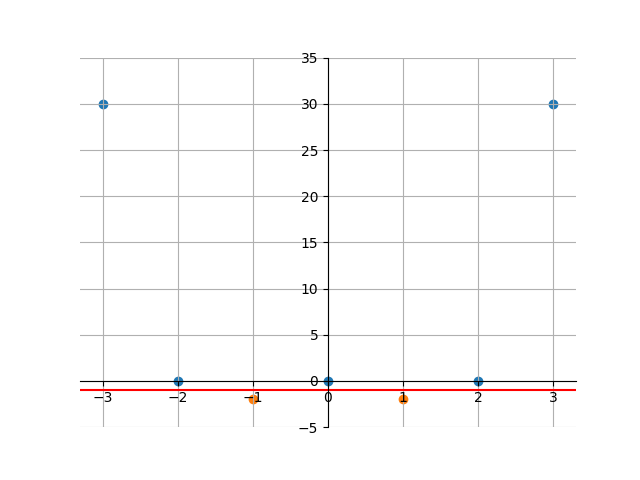
\includegraphics[scale=0.6]{1.1.png}
\end{center}

\noindent\textbf{Solution 1.2:}\\
The optimal decision boundary in 1.1 achieves a margin of 1.

\noindent\textbf{Solution 1.3:}\\
An unit vector orthogonal to the decision boundary is: $\boldw = \begin{bmatrix} 0 \\ 1 \\ \end{bmatrix}$.

\noindent\textbf{Solution 1.4:}\\
The optimal decision boundary exists where the discriminant equals 0:
\begin{align*}
    \boldw^\top \bphi(x) + w_0 &= 0
\end{align*}
Vectors on the decision boundary have the form, $\bphi(x) = \begin{bmatrix} 0 \\ \lambda \\ \end{bmatrix}$ (where $\lambda \in \reals$). Therefore, on the decision boundary, the discriminant can be written as:
\begin{align*}
    \boldw^\top \begin{bmatrix} 0\\ \lambda \\ \end{bmatrix} + w_0 &= 0\\
    \begin{bmatrix} w_1 \\ w_2 \\ \end{bmatrix}^\top \begin{bmatrix} 0\\ \lambda \\ \end{bmatrix} + w_0 &= 0\\
    w_2 \lambda = -w_0\\
    \lambda = -\frac{w_0}{w_2}
\end{align*}
In 1.1, we found that the decision boundary was given by $\bphi(x)_2 = -1$. Comparing this to the above expression, we get:
\begin{align*}
    -\frac{w_0}{w_2} &= -1 \text{on the decision boundary}\\
    \implies  w_2 &= w_0
\end{align*}
Therefore, $(\boldw, w_0) = (\begin{bmatrix} 0 \\ w_0 \\ \end{bmatrix}, w_0)$ (for all $w_0 \in \reals$) defines the set which makes the discriminant equal to 0.

\noindent\textbf{Solution 1.5:}\\
By inspection, the width between the support vectors (the vectors with the min margin) is 2. Given the expression for width between support vectors $\frac{2}{\|\mathbf{w}\|}$, and the $\boldw$ we found in 1.4, we can find the optimal $\boldw$:
\begin{align*}
    \frac{2}{\|\mathbf{w}\|} &= 2\\
    \frac{2}{\left\|\begin{bmatrix} 0\\ w_0 \\ \end{bmatrix}\right\|} &= 2\\
    \frac{2}{\sqrt{0^2 + w_0^2}} &= 2\\
    w_0 &= 1\\
\end{align*}
\begin{align*}
    \therefore \boldw^* = \begin{bmatrix} 0\\ 1 \\ \end{bmatrix}
\end{align*}

\noindent\textbf{Solution 1.6:}\\
From 1.4: $w_0^* = 1$.\\
Therefore, the discriminant function is $h(\bphi(x);\boldw^*,w_0^*) = \begin{bmatrix} 0\\ 1 \\ \end{bmatrix} \cdot \bphi(x) + 1 &= 0$.

\noindent\textbf{Solution 1.7:}\\
Support vectors exist anywhere on the lines $\bphi(x)_2 = 0$ and $\bphi(x)_2 = -2$, so they have the form $\begin{bmatrix} x_1\\ 0\\ \end{bmatrix}$ and $\begin{bmatrix} x_1\\ -2\\ \end{bmatrix}$ respectively. The constraint is tight when $y_i(\mathbf{w}^\top \bphi(x_i) + w_0) = 1$.

On $\bphi(x)_2 = 0$, $y_i = 1$:
\begin{align*}
    1\left(\begin{bmatrix} 0\\ 1\\ \end{bmatrix}^\top \begin{bmatrix} x_1\\ 0\\ \end{bmatrix} + 1\right) = 1(0+1) = 1
\end{align*}

On $\bphi(x)_2 = 0$, $y_i = -1$:
\begin{align*}
    1\left(\begin{bmatrix} 0\\ 1\\ \end{bmatrix}^\top \begin{bmatrix} x_1\\ -2\\ \end{bmatrix} + 1\right) = -1(-2+1) = 1
\end{align*}

Thus, the constraints are tight for all support vectors of the classifier. $\qedsymbol$

\noindent\textbf{Solution 1.8:}\\
As before, blue coordinates represent the transformed data with class $y = +1$; orange coordinates represent the transformed data with class $y = -1$. However, this feature map is clearly not linearly separable - there is no one straight line that separates the blue and orange points. Thus, for this SVM classification problem, I would choose to use the feature map plotted in part 1.1, as calculation of the margin is much simpler.
\begin{center}
    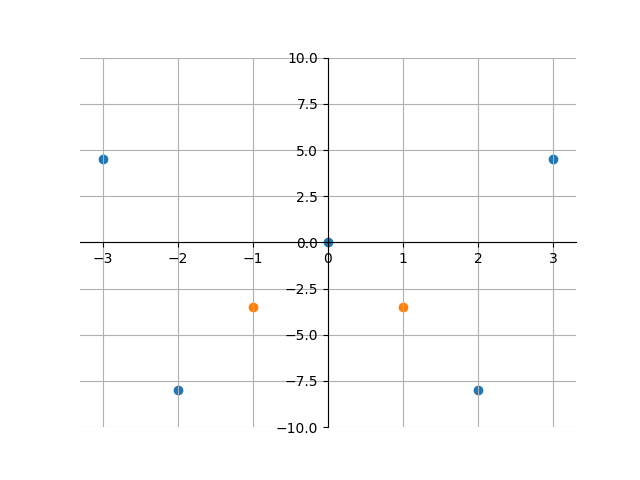
\includegraphics[scale=0.6]{1.8.png}
\end{center}

%%%%%%%%%%%%%%%%%%%%%%%%%%%%%%%%%%%%%%%%%%%%%
% Problem 2
%%%%%%%%%%%%%%%%%%%%%%%%%%%%%%%%%%%%%%%%%%%%%

\begin{problem}[K-Means and HAC, 20pts]

For this problem you will implement K-Means and HAC from scratch to cluster image data. You may use \texttt{numpy} but no third-party ML implementations (eg. \texttt{scikit-learn}).

We've provided you with a subset of the MNIST dataset, a collection of
handwritten digits used as a benchmark for image recognition (learn more at
\url{http://yann.lecun.com/exdb/mnist/}). MNIST is widely used in supervised learning, and modern algorithms do very well. 

You have been given
representations of MNIST images, each of which is a $784\times1$
greyscale handwritten digit from 0-9. Your job is to implement K-means and HAC on MNIST, and to test whether these relatively
simple algorithms can cluster similar-looking images together.

The code in \texttt{T4\_P2.py} loads the images into your environment into two arrays -- \texttt{large\_dataset}, a 5000x784 array, will be used for K-means, while \texttt{small\_dataset}, a 300x784 array, will be used for HAC. In your code, you should use the $\ell_2$ norm (i.e. Euclidean distance) as your distance metric.

\textbf{Important:} Remember to include all of your plots in your PDF submission!

\textbf{Checking your algorithms:} Instead of an Autograder file, we have provided a similar dataset, \texttt{P2\_Autograder\_Data}, and some visualizations, \texttt{HAC\_visual} and \texttt{KMeans\_visual}, for how K-means and HAC perform on this data. Run your K-means (with $K=10$ and \texttt{np.random.seed(2)}) and HAC on this second dataset to confirm your answers against the provided visualizations. Do \textbf{not} submit the outputs generated from \texttt{P2\_Autograder\_Data}. Load this data with \texttt{data = np.load(`P2\_Autograder\_Data.npy')}.

\begin{enumerate}

\item Starting at a random initialization and $K = 10$, plot the
  K-means objective function (the residual sum of squares) as a
  function of iterations and verify that it never increases.

\item For $K=10$ and for 3 random restarts, print the mean image (aka
  the centroid) for each cluster. There should be 30 total images. Code 
  that creates plots for parts 2, 3, and 4 can be found in \texttt{T4\_P2.py}.

\item Repeat Part 2, but before running K-means, standardize or center
  the data such that each pixel has mean 0 and variance 1 (for any
  pixels with zero variance, simply divide by 1). For $K=10$ and 3
  random restarts, show the mean image (centroid) for each
  cluster. Again, present the 30 total images in a single
  plot. Compare to Part 2: How do the centroids visually differ? Why?

\item Implement HAC for min, max, and centroid-based linkages. Fit
  these models to the \texttt{small\_dataset}.  For each of these 3
  linkage criteria, find the mean image for each cluster when using
  $10$ clusters. Display these images (30 total) on a single plot.

  How do the ``crispness'' of the cluster means and the digits
  represented compare to mean images for k-means?  
  Why do we only ask you to run HAC once?  

  \textbf{Important Note:} For this part ONLY, you may use
  \texttt{scipy}'s \texttt{cdist} function to calculate Euclidean
  distances between every pair of points in two arrays.

\item For each of the HAC linkages, as well as one of the runs of your
  k-means, make a plot of ``Number of images in cluster" (y-axis)
  v. ``Cluster index" (x-axis) reflecting the assignments during the
  phase of the algorithm when there were $K=10$ clusters.

  Intuitively, what do these plots tell you about the difference
  between the clusters produced by the max and min linkage criteria?

  Going back to the previous part: How does this help explain the
  crispness and blurriness of some of the clusters?  
\end{enumerate}
\end{problem}

\newpage
\begin{framed}
\noindent\textbf{Problem 2} (cont.)\\
\begin{enumerate}
\setcounter{enumi}{5}
\item For your K-means with $K = 10$ model and HAC min/max/centroid
  models using $10$ clusters on the \texttt{small\_dataset} images,
  use the \texttt{seaborn} module's \texttt{heatmap} function to plot
  a confusion matrix between each pair of clustering methods.  This
  will produce 6 matrices, one per pair of methods. The cell at the
  $i$th row, $j$th column of your confusion matrix is the number of
  times that an image with the cluster label $j$ of one method has
  cluster $i$ in the second method.  Which HAC is closest to k-means?
  Why might that be?

\item Suppose instead of comparing the different clustering methods to
  each other, we had decided to compute confusions of each clustering
  method to the \emph{true} digit labels (you do \emph{not} have to
  actually compute this).  Do you think how well the clustering match
  the true digits is reasonable evaluation metric for the clustering?
  Explain why or why not.
  
\end{enumerate}
\end{framed}


\subsection*{Solution}
\noindent\textbf{Solution 2.1:}\\
The plot verifies that the K-means objective function is always decreasing as the number of iterations increases:
\begin{center}
    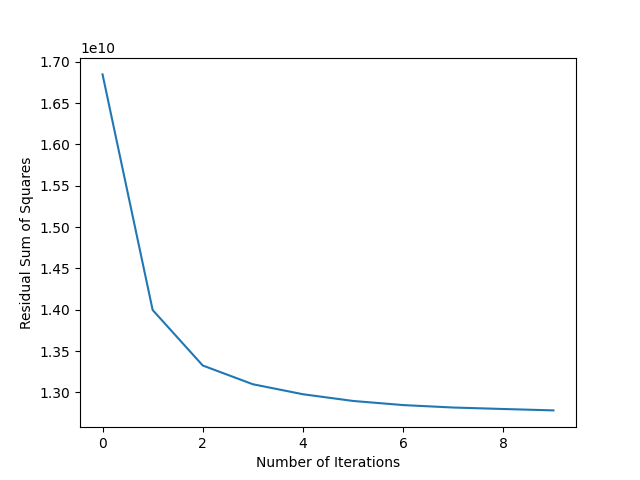
\includegraphics[scale=0.7]{2.1.png}
\end{center}
\newpage

\noindent\textbf{Solution 2.2:}\\
\begin{center}
    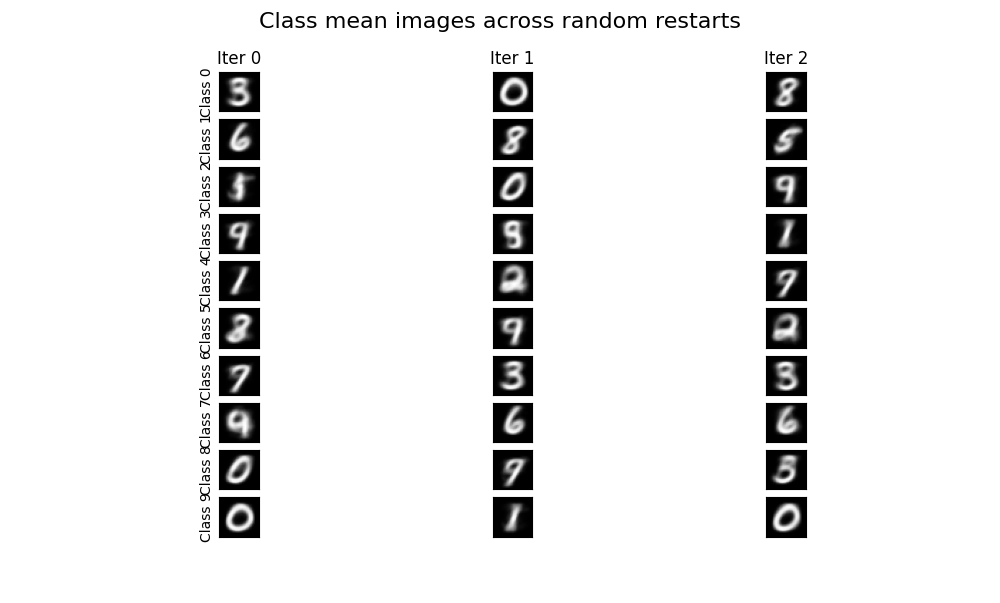
\includegraphics[scale=0.6]{2.2.png}
\end{center}

\noindent\textbf{Solution 2.3:}\\
\begin{center}
    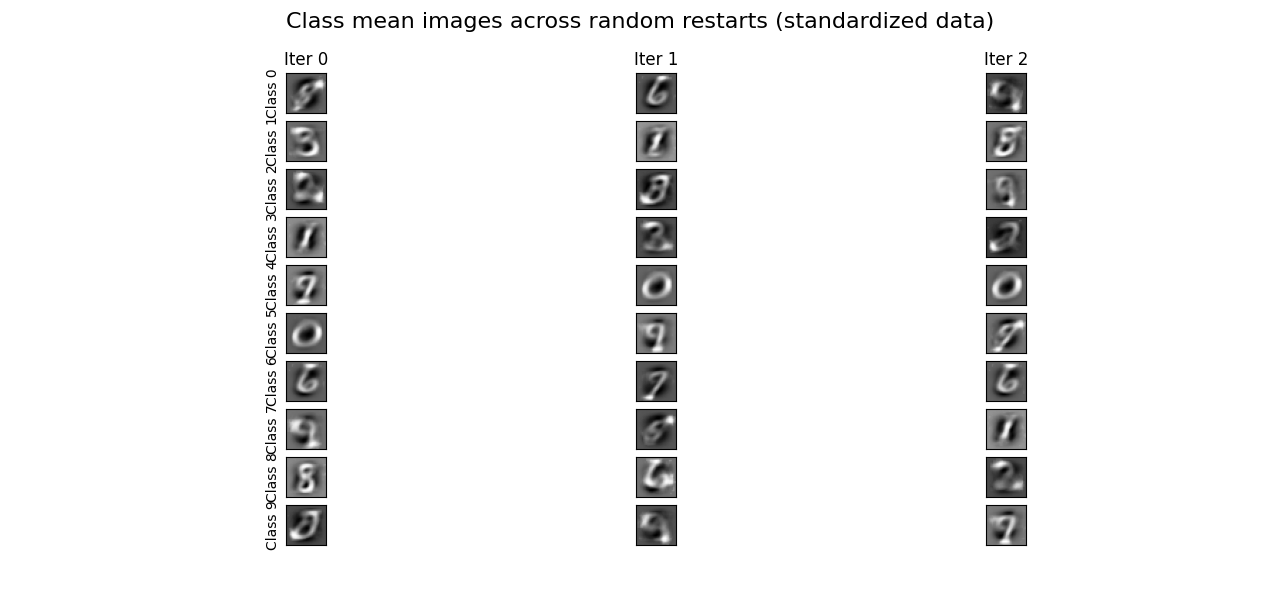
\includegraphics[scale=0.6]{2.3.png}
\end{center}
All of the pixels in the mean images (the centroids) appear to be greyer, rather than a crisp black background with white colored text overlayed as seen in 2.2. As a result, the images created from standardized data appear blurrier.\\

This occurs because pixel values range from 0 (white) to 255 (black). If you consider an edge pixel in the image, which is usually black-ish, it will have a pixel value $>$200. Thus, the mean of an edge pixel is ~227.5. Therefore, where we standardize an edge pixel that is pure black, the pixel value becomes $\frac{(255 - 227.5)}{\sigma_i} = \frac{(27.5)}{\sigma_i}$. This standardized pixel value is significantly lower than the original, so the edge pixel appears lighter/greyer. Analogously, if you consider a central pixel in the image, which is usually white-ish, it will have a pixel value $<$50. Thus, the mean of an edge pixel is ~22.5. Therefore, where we standardize a central pixel that is pure black, the pixel value becomes $\frac{(50 - 22.5)}{\sigma_i} = \frac{(22.5)}{\sigma_i}$. This standardized pixel value is again lower than the original, so the central pixel appears lighter/greyer.\\

Ultimately, therefore, the pixels are all lighter and are end up being more similar in color. This makes sense, given the pixels in our standardized images have a lower variance than in the originals (which have high contrast between black and white pixels).

\noindent\textbf{Solution 2.4:}\\
\begin{center}
    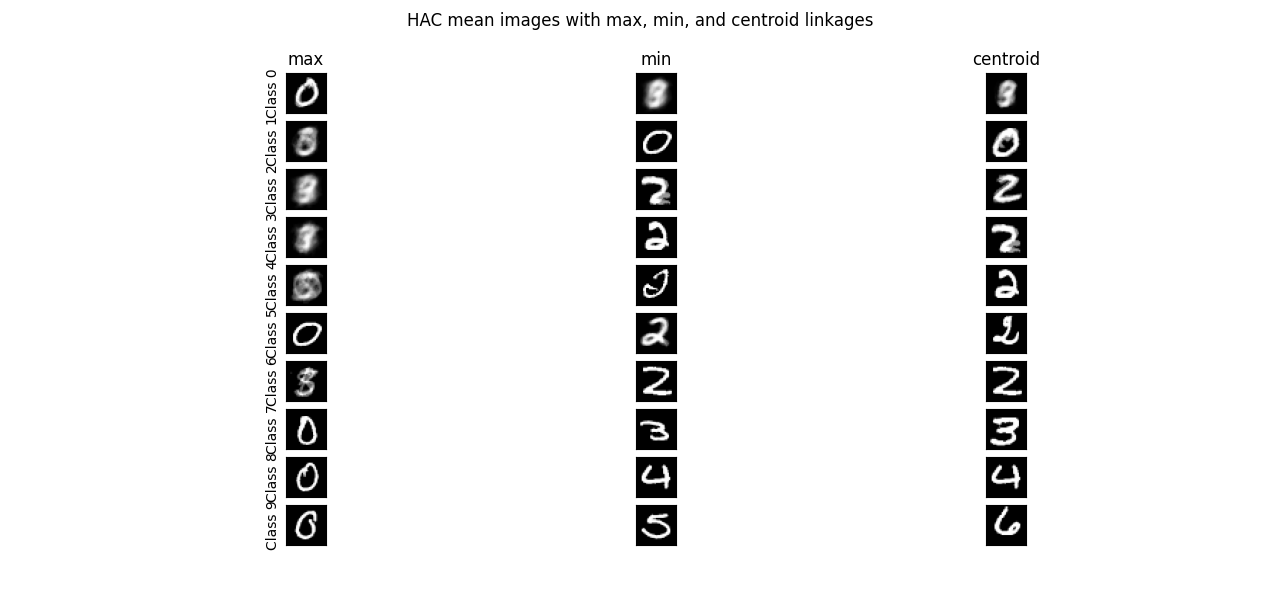
\includegraphics[scale=0.6]{2.4.png}
\end{center}
The crispness of the k-means images was quite high (for the non-standardized data). The HAC max cluster means appear to be the blurriest, whilst the HAC min and HAC centroid cluster means appear quite crisp in all but the first (0th) class.\\

Unlike k-means, which needs to be run several times in order to avoid ``getting stuck" at a local minimum of the objective function, HAC only needs to be run once, after having selected a linkage criterion, because it calculates the clusters in a deterministic way (without using calculus).

\noindent\textbf{Solution 2.5:}\\
\begin{center}
    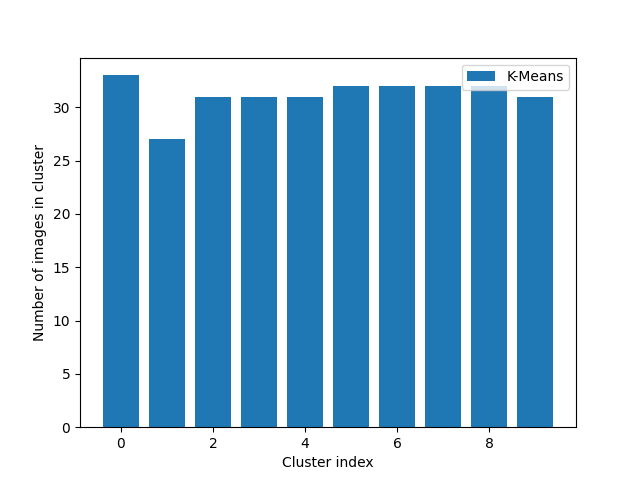
\includegraphics[scale=0.6]{HW4/2.5_kmeans.png}
\end{center}
\begin{center}
    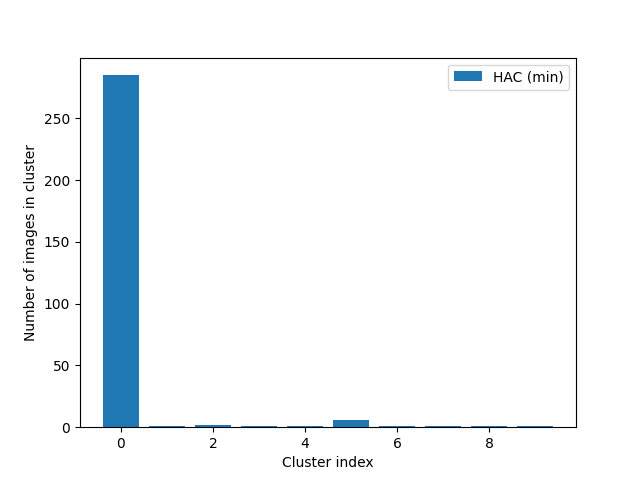
\includegraphics[scale=0.6]{HW4/2.5_hacmin.png}
\end{center}
\begin{center}
    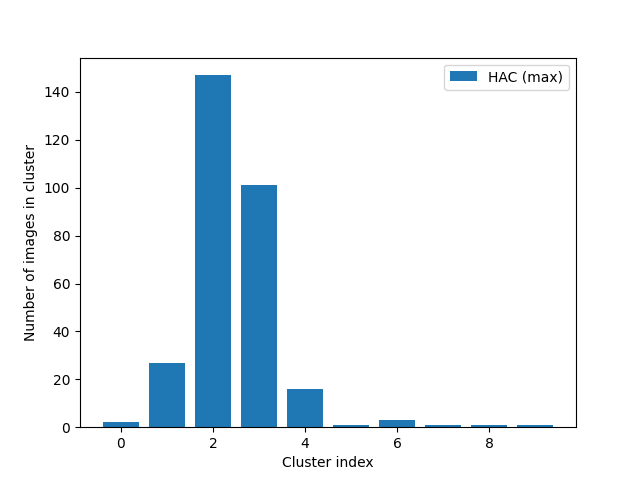
\includegraphics[scale=0.6]{HW4/2.5_hacmax.png}
\end{center}
\begin{center}
    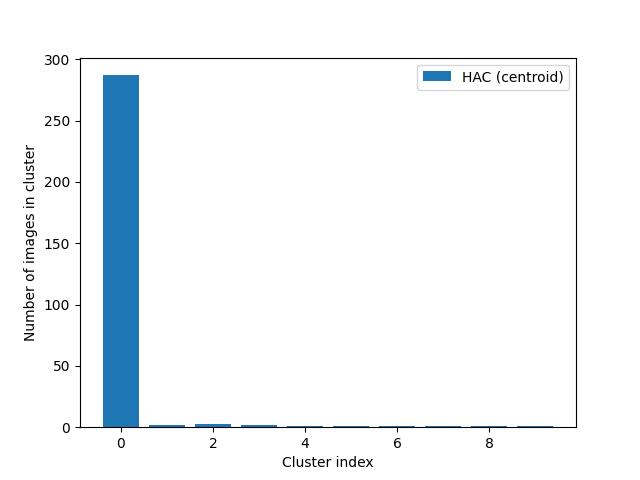
\includegraphics[scale=0.6]{HW4/2.5_haccentroid.png}
\end{center}
HAC min and HAC centroid seem to cluster most images into a single cluster, whilst HAC max clusters images across a broader range of clusters. Intuitively this makes sense: for min, when a cluster gets larger, the probability that this cluster is close to other clusters increases, increasing the likelihood that this large cluster increases in size again; for max, when a cluster gets larger, it gets closer to other larger sized clusters, and so the next max distance is unlikely to be in another already-large cluster, so the likelihood of the large cluster increasing in size again decreases. This explains why max-linkage produces compact clusters, while min-linkage latches onto any neighboring closest cluster and produces stringy clusters.\\

The blurriness of the outputs can be explained when a cluster mean is the average of many outputs, e.g. HAC max is quite blurry in many classes because there are lots of images in many of the classes; HAC min and HAC centroid have blurry outputs for class 0, but relatively crisp outputs for the other classes, which are averaging relatively few images; k-means is very crisp because there are only c. 30 (very few) images per class (an almost perfectly uniform distribution across clusters).
\newpage

\noindent\textbf{Solution 2.6:}\\
\begin{center}
    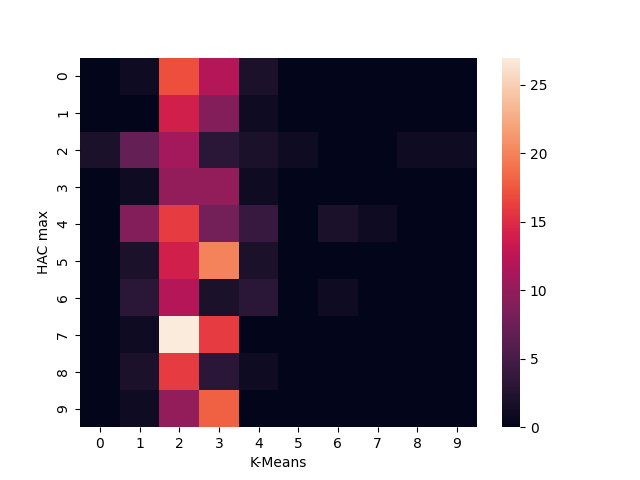
\includegraphics[scale=0.5]{HW4/2.6.1.png}
\end{center}
\begin{center}
    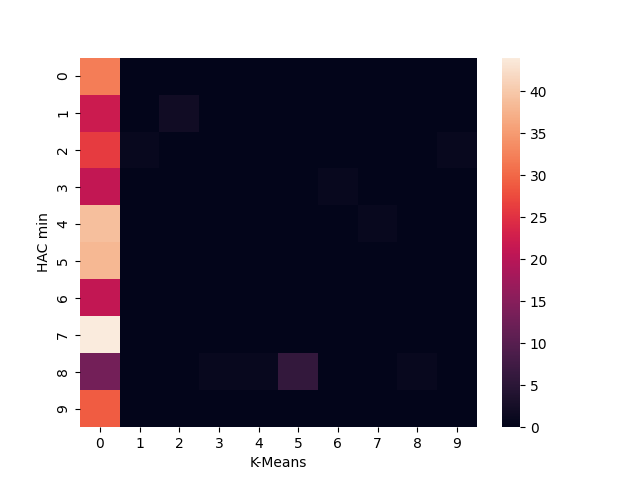
\includegraphics[scale=0.5]{HW4/2.6.2.png}
\end{center}
\begin{center}
    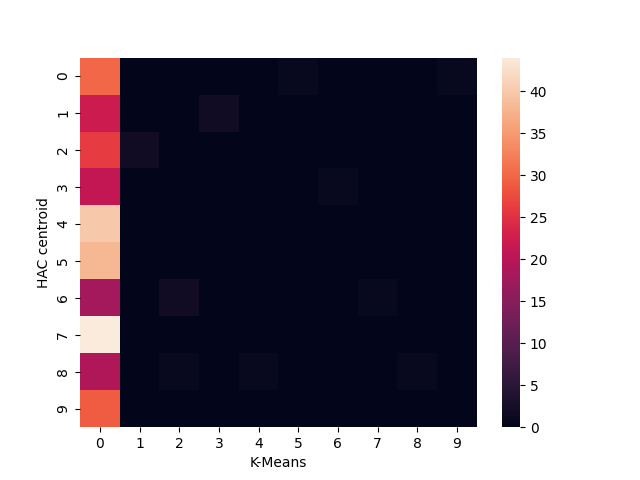
\includegraphics[scale=0.5]{HW4/2.6.3.png}
\end{center}
\begin{center}
    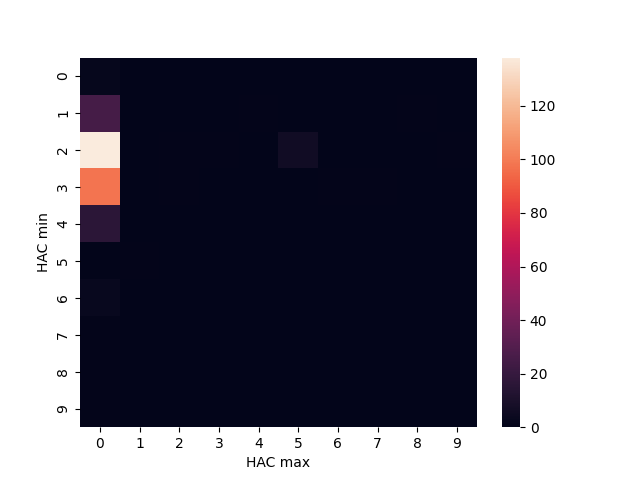
\includegraphics[scale=0.5]{HW4/2.6.4.png}
\end{center}
\begin{center}
    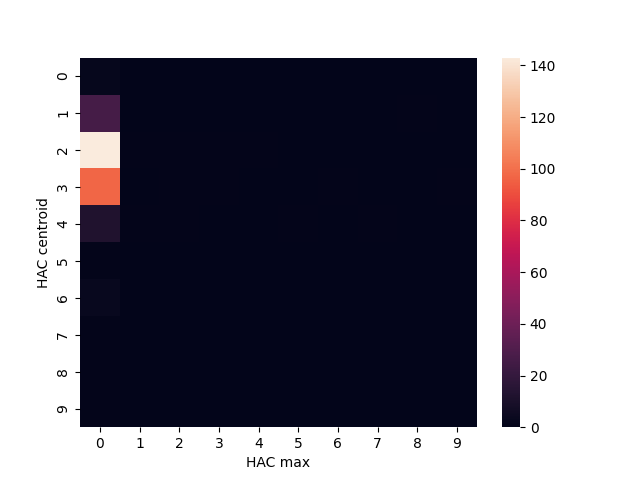
\includegraphics[scale=0.5]{HW4/2.6.5.png}
\end{center}
\begin{center}
    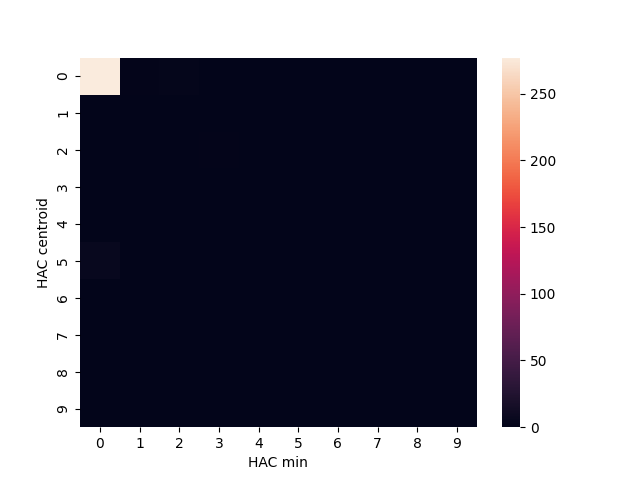
\includegraphics[scale=0.5]{HW4/2.6.6.png}
\end{center}
Based on the heatmaps , HAC max appears to be closest  to k-means. This seems to be because the max-linkage distributes images across classes more evenly than HAC min and HAC centroid, which is similar to the way k-means distributes images across classes, as also seen in the ``num. images in cluster plots" in 2.5. Thus, we see ``hotter" points distributed across more of the HAC max/k-means heatmap than other heatmaps.
\newpage

\noindent\textbf{Solution 2.7:}\\
Yes - how well the clustering matches the true digits is reasonable evaluation metric for the clustering. The more accurate the clusterings, the more we would see ``hotter" cells distributed evenly across our heatmaps; by comparison, less correct clusterings would produce uneven heatmaps. Effectively, using the true digits to evaluate the clustering turns this problem into a supervised learning problem, rather than an unsupervised one - e.g. we could use something like 0/1 loss as a basic evaluation metric using such a method.

\newpage
%%%%%%%%%%%%%%%%%%%%%%%%%%%%%%%%%%%%%%%%%%%%%
% Problem 3
%%%%%%%%%%%%%%%%%%%%%%%%%%%%%%%%%%%%%%%%%%%%%

\begin{problem}[Ethics Assignment, 5pts]

Select a real-life outcome in Artificial Intelligence or Machine Learning 
that you believe is morally wrong. You can select your own outcome from 
the news or select one of the outcomes in the options below:

\begin{itemize}
    \item COMPAS, a case management tool predicting recidivism that 
        flagged “blacks are almost twice as likely as whites to be 
        labeled a higher risk but not actually re-offend” (Angwin 
        2016).
        
    \item An NLP algorithm filled in the inference “Man is to 
        \_\_\_\_ as woman is to \_\_\_\_” with “Man is 
        to computer programmer as woman is to homemaker” (Bolukbasi 
        et al, 2016).
        
    \item \url{http://www.survivalofthebestfit.com/game}: a game that 
        exemplifies algorithmic bias in resume screening
        
    \item IBM Diversity in faces: insufficient training data for 
        darker-skinned faces
        
    \item Other Unfair Algorithms: Algorithms of Oppression (a really 
        good book with tons of examples), VI-SPDAT, Allegheny Family 
        Screening Tool
        
\end{itemize}
Draw a causal chain that resulted in this outcome and circle the choice points that were the largest contributors to the outcome. At each morally relevant choice point, write two alternative decisions that could have prevented the outcome.

\end{problem}

\subsection*{Solution}

\newpage
%%%%%%%%%%%%%%%%%%%%%%%%%%%%%%%%%%%%%%%%%%%%%
% Name and Calibration
%%%%%%%%%%%%%%%%%%%%%%%%%%%%%%%%%%%%%%%%%%%%%
\subsection*{Name}

\subsection*{Collaborators and Resources}
Whom did you work with, and did you use any resources beyond cs181-textbook and your notes?\\
https://www.cs.princeton.edu/courses/archive/fall18/cos324/files/kmeans.pdf\\
Josh Michels, Elias Nuwara, Ty Geri\\

Did you attend office hours for help with this homework?\\
Yes

\subsection*{Calibration}
Approximately how long did this homework take you to complete (in hours)?\\
18

\end{document}